\documentclass[a4paper,14pt]{extarticle}
\usepackage{geometry}
\usepackage{fullpage}
\usepackage[parfill]{parskip}
\usepackage{graphicx}
\usepackage{tikz}
\begin{document}
\begin{center}
\LARGE{MECH 4450 Term Project Report}\\\vspace{1em}
\Large{Project 2 (Static structure)}\\\vspace{1em}
\Large{Kong Xiangzhou 20026414}\\\vspace{1em}
\end{center}
\section{Introduction}
TODO
\section{Program modelling}
\subsection{Geometry}
The top view of original design is shown below:

\begin{center}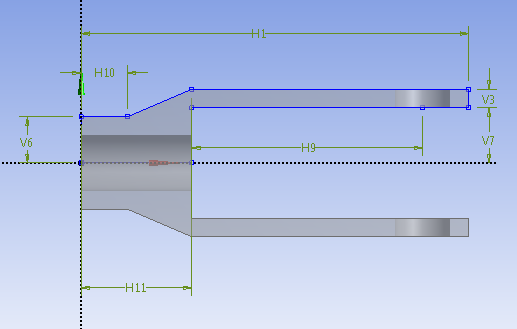
\includegraphics[width=0.75\textwidth]{2D_ORIGIN.png}\end{center}

Where $H1=42cm$, $H10=5cm$, $H11=12cm$, $H9=25cm$, $V3=2cm$, $V6=5cm$, $V7=6cm$, diameters of all holes are $6cm$.

It is resembled as below:

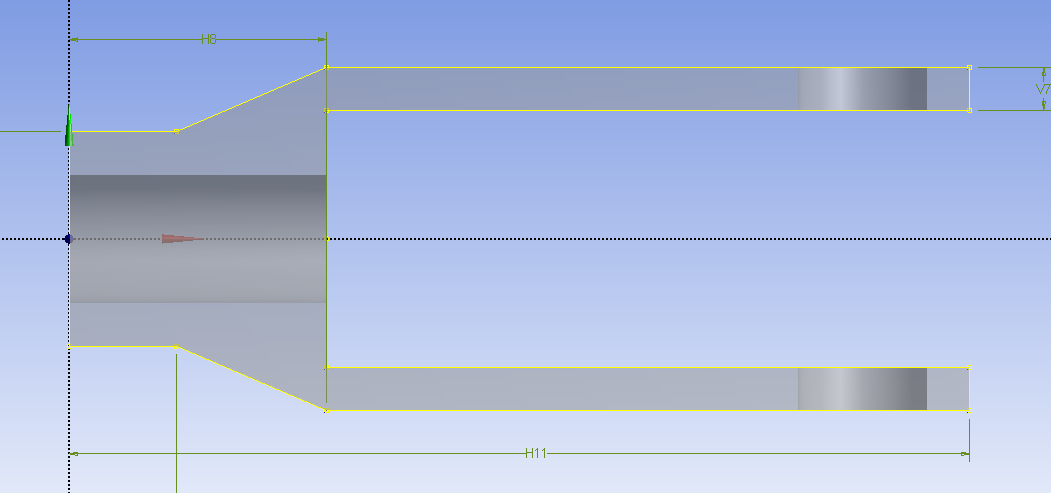
\includegraphics[width=\textwidth]{2D_S_01.PNG}

The 3D model built is then as below, where the height of the component is assumed to be $10 cm$:

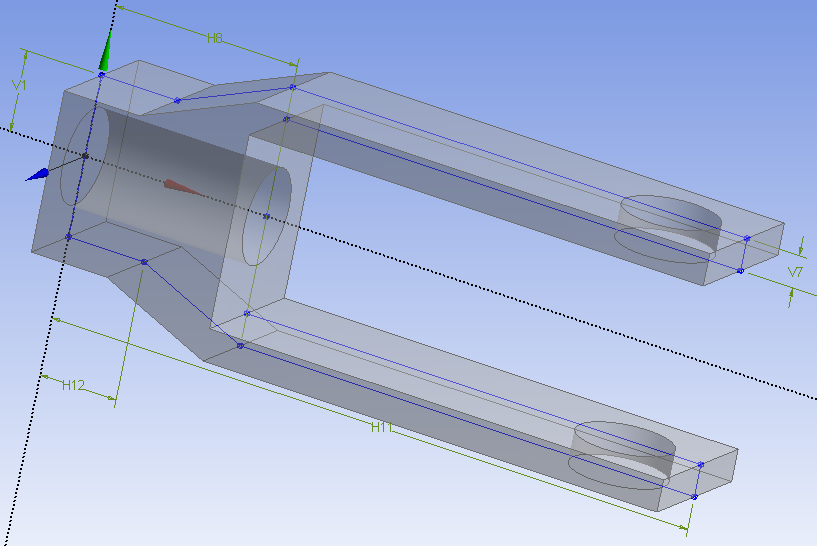
\includegraphics[width=\textwidth]{3D_S_01.PNG}

The boundary conditions are the loads, where symmetric properties on both axis can be assumed.
\section{FEM analysis}
\subsection{Mesh setup}
For the mesh, two refinements are added as below, where the first one (\textit{Refinement}) is for the cylindrical surface of loading, and the second one (\textit{Refinement 2}) is for the sharp edges of 90 degree where stress concentration might occur.

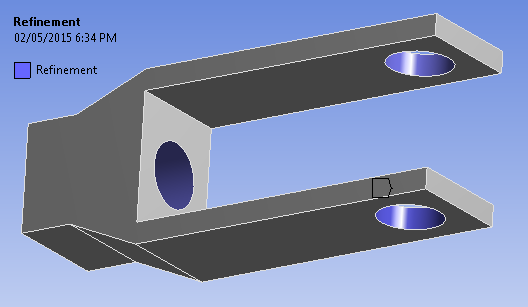
\includegraphics[width=0.5\textwidth]{REF1.PNG}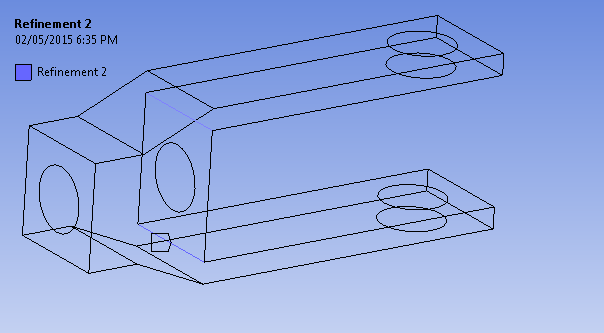
\includegraphics[width=0.5\textwidth]{REF2.PNG}

The overall mesh with a size of $2cm$ is shown below:

\includegraphics[width=0.5\textwidth]{{MESH_0.02}.PNG}\includegraphics[width=0.5\textwidth]{{MESH_0.02F}.PNG}
\subsection{Boundary conditions setup}
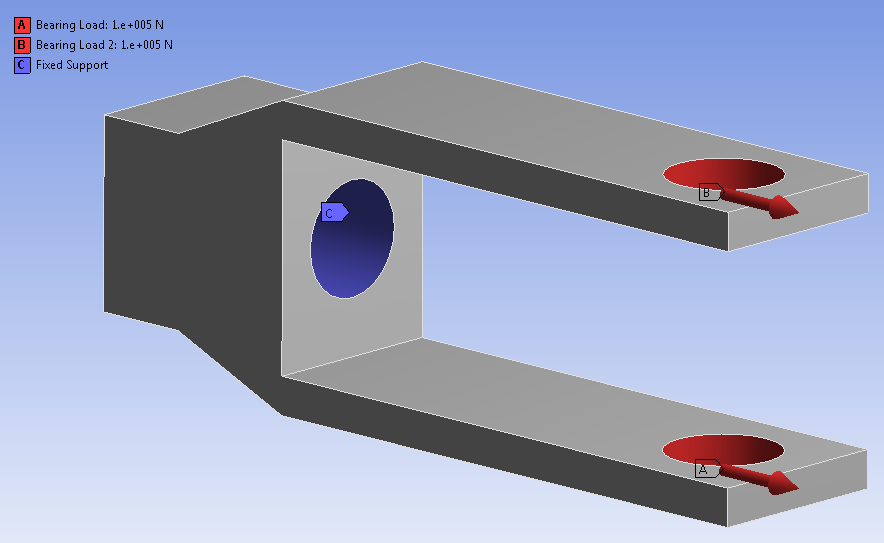
\includegraphics[width=\textwidth]{Model.PNG}
\subsection{Convergence study}
For convergence study, mesh sizes of  $3cm$, $2cm$, $1.5cm$m $1cm$, $0.8cm$ and $0.65cm$ are used. The mesh of minimum ($0.65cm$) and maximum ($3cm$) mesh size are shown below:

\includegraphics[width=0.5\textwidth]{{MESH_0.0065}.PNG}\includegraphics[width=0.5\textwidth]{{MESH_0.03}.PNG}

The results for principle stresses are below, listed in size-decreasing order.

\includegraphics[width=0.5\textwidth]{{STRESS_0.03}.PNG}\includegraphics[width=0.5\textwidth]{{STRESS_0.02}.PNG}
\includegraphics[width=0.5\textwidth]{{STRESS_0.015}.PNG}\includegraphics[width=0.5\textwidth]{{STRESS_0.01}.PNG}
\includegraphics[width=0.5\textwidth]{{STRESS_0.008}.PNG}\includegraphics[width=0.5\textwidth]{{STRESS_0.0065}.PNG}

The results for deformations are below, listed in size-decreasing order.

\includegraphics[width=0.5\textwidth]{{DEFORM_0.03}.PNG}\includegraphics[width=0.5\textwidth]{{DEFORM_0.02}.PNG}
\includegraphics[width=0.5\textwidth]{{DEFORM_0.015}.PNG}\includegraphics[width=0.5\textwidth]{{DEFORM_0.01}.PNG}
\includegraphics[width=0.5\textwidth]{{DEFORM_0.008}.PNG}\includegraphics[width=0.5\textwidth]{{DEFORM_0.0065}.PNG}

The change of both results with mesh sizes can be plotted below (x-axis in reciprocal scale):

\begin{center}
\begin{tikzpicture}[y=20, x=20]
	\tikzstyle{every node}=[font=\footnotesize]

 	%axis
	\draw (0,0) -- coordinate (x axis mid) (20,0);
    	\draw (0,0) -- coordinate (y1 axis mid) (0,10);
    	\draw (20,0) -- coordinate (y2 axis mid) (20,10);
    	
    	%ticks
    	\foreach \x in {0.0065,0.008,0.01,0.015,0.02,0.03}
		\draw ({0.1 / \x},0) -- ({0.1 / \x},0.2)
			node[anchor=south] {\x};
    	\foreach \y in {2,4,...,10}
    		\pgfmathtruncatemacro{\val}{\y *10 + 400}%
		\draw (0,\y) -- (0.2,\y) 
     			node[anchor=west] {\val}; 
    	\foreach \y in {2,4,...,10}
		\pgfmathtruncatemacro{\val}{(\y / 15 + 39) * 100}%
		\draw (20,\y) -- (19.8,\y) 
     			node[anchor=east] {\val}; 
     	
	%labels      
	\node[below=0.5] at (x axis mid) {Mesh size / $cm$};
	\node[red,rotate=90, above=0.5] at (y1 axis mid) {Max. principle stress / $MPa$};
	\node[blue,rotate=-90, above=0.5] at (y2 axis mid) {Max. deformation / $10^{-7}m$};

	%plots
	\draw[red] ({0.1 / 0.03},{(4.2957 - 4) * 10})  --  ({0.1 / 0.02},{(4.5612 - 4) * 10}) -- ({0.1 / 0.015},{(4.7094 - 4) * 10}) -- ({0.1 / 0.011},{(4.75 - 4) * 10}) --  ({0.1 / 0.008},{(4.7325 - 4) * 10}) -- ({0.1 / 0.0065},{(4.7684 - 4) * 10});
	\draw[blue] ({0.1 / 0.03},{(39.225 - 39) * 15}) --  ({0.1 / 0.02},{(39.36 - 39) * 15}) -- ({0.1 / 0.015},{(39.449 - 39) * 15}) -- ({0.1 / 0.011},{(39.485 - 39) * 15}) --  ({0.1 / 0.008},{(39.504 - 39) * 15}) -- ({0.1 / 0.0065},{(39.52 - 39) * 15});
\end{tikzpicture}
\end{center}

We can see it converges. Therefore using a mesh size of $0.65 cm$ in the following study will be reasonable.

\end{document}